In this chapter the project is planned in general. Currently the team is not in a position where it would be able to create a detailed plan for each sprint, so the following sections serve the purpose of a rough plan for the whole project. After finishing a preliminary studies some decisions about methodology tools, technology, collaboration, and a rough project plan were made. Planning increases the efficiency and it reduces the risks involved. It also facilitates proper coordination within a development team, and this will help us maintain a good control. Planning will help the team to achieve the goals by using the available time and resources, and of course planning helps in decision making  

\section{Work breakdown structure}
\label{sec:wbs}
The whole project was thoroughly examined  considering the stated scope and the objectives and it was decomposed into eight main distinctive modules:

\begin{itemize}
\item Pre-study
\item Requirements elicitation
\item Project planning
\item Application design
\item Application implementation
\item Testing and evaluation
\item Project management
\item Documentation
\end{itemize}

The main modules can be further decomposed into smaller actions. The graphical representation of the whole work breakdown structure can be found in the appendix in chapter \ref{txt:work_breakdown_structure}.

\section{Organization}
This chapter outlines how the project group is organized and why.
To perform efficiently and effectively it is important to figure out what kind of organizational structure is suitable. 
Structures provides an overview of who makes decisions and is responsible, how information flows within and between organizational units and suggests what it takes to move between departments. This means that a good organizational structure provides the team with the clarity of the different responsibilities. Since one of the goals is to finish the project in the given time frame it is important to have a good organizational structure.

\begin{table*}\centering \ra{1.3}
    \caption[Skills and previous experience]{Skills and previous experience table. Coding:
        \textcolor{green!100}{$\bullet$} expert,
        \textcolor{green!60}{$\bullet$} experienced,
        \textcolor{yellow!75}{$\bullet$} neutral,
        \textcolor{orange!90}{$\bullet$} little experience,
        \textcolor{red!80}{$\bullet$} no experience}
    \label{tab:skills}
    \vspace{2mm}
    \begin{tabular}{lcccc}
    \toprule[0.5mm]
                                & Agnethe   & Tomas & Milos & Jan \\
    \midrule
    \textbf{Leadership                 } & \colorB & \colorE & \colorD & \colorC \\ 
    \textbf{Scrum                      } & \colorB & \colorE & \colorE & \colorE \\ 
    \textbf{Mobile software development} & \colorC & \colorE & \colorB & \colorE \\ 
    \textbf{\LaTeX                     } & \colorE & \colorB & \colorE & \colorB \\ 
    \textbf{Network programming        } & \colorD & \colorC & \colorC & \colorC \\ 
    \textbf{Image processing           } & \colorE & \colorC & \colorE & \colorD \\ 
    \textbf{Java                       } & \colorC & \colorD & \colorA & \colorE \\ 
    \textbf{C++                        } & \colorE & \colorB & \colorC & \colorB \\ 
    \textbf{Testing                    } & \colorE & \colorB & \colorD & \colorC \\
    \bottomrule[0.5mm]
    \end{tabular}
\end{table*}

\subsection{Role Assignment}
To assign roles according to members' skills and previous experience it was decided to make a survey of relevant knowledge. 
Results of this survey can be seen in Table \ref{tab:skills}. 
This table was used as a base for the role assignment.
In the beginning, during planning, not so many roles were establish, but during the development process itself it was found out that some of them are necessary. 
Nevertheless only few roles are used and the responsibility of unused roles (mentioned in compendium) are distributed to all members. 
The bottom line is that as a development team all of the members are equal.
The assigned roles can be seen in Table \ref{tab:roles}. 

\begin{table*}\centering \ra{1.3}
    \caption{Assigned roles and their responsibilities}
    \label{tab:roles}
    \vspace{2mm}
    \begin{tabularx}{\textwidth}{llX}
    \toprule[0.5mm]
    Role    & Person   & Responsibility \\
    \midrule
    \textbf{Project Leader}             & Agnethe &
        Responsible for progress of the project according to the plan.
        Distributes work to group members.
        Has final call in arguments.\\
    \textbf{System Architect}             & Milos &
        Check consistency and analyze all layers of the product. \\
    \textbf{Scrum Master}             & Agnethe &
        Leads the scrum stand-ups. \\
    \textbf{Communication Responsible}  & Jan &
        Responsible for communicating with customer and supervisor.
        Regularly send meeting minutes, agenda and other documents to customer and supervisor. \\ 
    \textbf{QA Responsible} & Tomas &
        Ensure a quality of all documents and end-product.        \\ 
    \textbf{Documentation Responsible} & Agnethe &
        Responsible for delegating and supervising work on final report.        \\         
    \bottomrule[0.5mm]
    \end{tabularx}
\end{table*}

\section{Risk Management}
In the Table \ref{tab:risks} the consequence and possibility in a number between 1--10. The risk, or the riskfactor, is the consequence multiplied with the possibility. The risks in this table is very obvious ones. 

Other risks can be seen from analyzing the skill table. If for example the only two persons on the team who are familiar with image processing are not present, then this will be a risk. There is a great possibility that this kind of task will take longer time then planned for. 

Also if some of the rows in the skill table all were painted red, which  would imply that the team had no experience with this, then this would be a risk. 
In such a case, studying of that field of area would have to start immediately and a meeting with the customer should be planned about considering scaling down the task.

\begin{sidewaystable}
    \caption{Handling risks}
    \label{tab:risks}
    
    \centering \ra{1.3}
    \vspace{2mm} %\rotatebox{90}{
    \begin{tabularx}{500pt}{XcccXX}
    \toprule[0.5mm]
        Event & Consequence & Possibility & Risk  & Reactive Measures & Proactive Measures \\
    \midrule
Someone gets sick & 4     & 5     & 20    & Other people do more work.  & Free weekends \\
Coding problems & 4     & 7     & 28    & Talk to supervisor and/or relevant persons & preparing for the task \\
Testing problems & 4     & 4     & 16    & Talk to customer about reformulating requirements & Double check requirements with customer \\
Implementing things we are not supposed to & 7     & 6     & 42    & Try to adopt functionality or start all over & Don't do anything that is not in backlog and keep good communication with customer \\
Dead end with technologies & 8     & 8     & 64    & Talk to supervisor \& Guru office & Do thoroughly research \\
Unrealistic time estimate & 7     & 8     & 56    & Work overtime  & Planing poker \\
Frequent changes in requirements specification & 6     & 3     & 18    & Renegotiate with a customer & Try no to change finished modules and keep weekly meetings with the customer \\
Customer too ambitious & 9     & 5     & 45    & Renegotiate with a customer & Keep customer informed about what  to expect \\
Hardware problems & 9     & 3     & 27    & Obtain a new one & Keep your devices updated \\
\bottomrule[0.5mm]
\end{tabularx}
\end{sidewaystable}

\label{sec:limitations}
This project is developed under a few technical, resource, time and knowledge limitations. 

The biggest limitation is the image processing part. Half of the team has no experience with this, and the other half has little experience. Their experience is mostly theoretical information about the subject, and practical experience is preferred. This limitation is known to the team, and the plan is to learn by doing. This approach is chosen so that the team would no spend more time than necessary doing research.

Another limitation is lack of experience with mobile development within the development team. All of the team members have Android phones, and to be able to test our application, an Android application must be developed. Only one team member has experience with this. 

If the project is not scaled down, the system could not be tested as the required resources are not available. Numerous audience, dozens of Android phones or big screen is a good example.

As this course last for a 13 weeks, it is normal that some trade-offs must be made.
This project is technically difficult, and there is a limited amount of time. 


\section{Communication}
Specific guidelines and practices were adopted so that the team and the customer could continuously verify that the project development keeps the right direction and that the requirements are being fulfilled.

\subsection{Customer collaboration}
Since the scope of the project and the actual requirements are determined by the customer it is essential to establish tight collaboration practices and even involve the customer in the collaboration tools the team uses. The description of our approach to fulfilling sufficient customer relations follows.

\paragraph{Meetings}
It has been agreed that weekly meetings taking approximately 60 minutes will be held. The standard agenda consists of the approval of the meeting minutes summarizing the last meeting, comments on the meeting minutes and the specific issues regarding the team-customer collaboration and technical issues. As the customer is located in Oslo the meetings will be carried out using the video-conference devices provided by the NTNU (accessible in the Accenture Lab). Contents of each meeting including the topics discussed, decisions made and the future plans are summarized in the meeting minutes. The team should provide the customer with the meeting minutes document before the next meeting is held.

\paragraph{Software tools}
As mentioned earlier the team decided to utilize the Target Process 3 as a collaboration tool suitable for handling Scrum-driven projects. The customer was invited to join the framework so that he could observe the development process more closely. Thanks to the software tool the customer is able to easily adjust the order of the user stories according to his preferences. the customer was also invited to the file sharing service and version control system that the team uses to save and distribute the documents and the source code.

\subsection{Supervisor collaboration}
It has been agreed on weekly meetings also with supervisor, at least from the beginning of the course.
These meetings are for the team to ensure that the right track is followed and also for the supervisor to be updated with team's progress.

If urgent situation occurs, supervisor will be contacted via email with detail of problem or with invitation for premature meeting.

\subsection{Team collaboration}
Mostly during the pre-study phase the developers need to distribute and maintain the information considered important for the next work. As stated in section \ref{sec:communication_tools} the Facebook group was chosen and set up to serve this purpose as it disposes of the tools suitable for exchanging website links, opinions and multimedia.

It has been also decided that the project report should be written continuously by all members as a part of our daily workflow. Through this practice the team will be able to keep track of the amount of work done and all members will make sure they understand well what direction the project is aiming.

\section{Duration and workload}
\label{sec:duration_and_workload}
Compendium proposed week workload 25 person-hours per week. 
During our internal meeting it was decided that each member will spend 30 hours per week because the team consists only of 4 members. 
Fixed daily working hours were suggested so that the workload could be distributed through the whole semester.
Regular stand-ups will be made according to Scrum methodology.

According to work break down structure \ref{sec:wbs} and presented week workload, initial time estimation of whole project was created. 
You can see the estimation in Table \ref{tab:initial-time-estimation}. 
As a part of a evaluation, spent hours will be filled, and then retrospective to the planning phase can be done.

\begin{table*}[!h]
	\caption{Initial time estimation table}
	\label{tab:initial-time-estimation}
	\def\arraystretch{1.25}
	\begin{tabularx}{\textwidth}{Xcccc}
		\toprule[0.5mm]
		\multirow{2}{*}{\textbf{Task}} &
		\multirow{2}{*}{\textbf{From date}} & 
		\multirow{2}{*}{\textbf{To date}} & 
		\multicolumn{2}{c}{\textbf{Hours}} \\
 				& & & \textbf{Estim.} & \textbf{Spent} \\
		\midrule
		Pre-study 					& 26.08.2013 & 15.09.2013 & 70 &  ?\\
		Requirements elicitation 	& 26.08.2013 & 29.09.2013 & 80 &  ?\\
		Project planning			& 26.08.2013 & 15.09.2013 &	75 &  ?\\
		Application design 			& 26.08.2013 & 27.10.2013 & 90 &  ?\\
		Application implementation	& 02.09.2013 & 20.11.2013 &	450 &  ?\\
		Testing and evaluation 		& 02.09.2013 & 20.11.2013 & 130 &	?\\
		Project Management  		& 26.08.2013 & 20.11.2013 & 120 &  ?\\
		Documentation				& 26.08.2013 & 20.11.2013 &	425 &  ?\\
		\midrule		
		\textbf{$\sum$}	& &	&		1440	& \textbf{?} \\								
		\bottomrule[0.5mm]
	\end{tabularx}
\end{table*}


\section{Project scope}
After third meeting with our customer it was decided to lay out the scope of the project that is tangible and doable under 13 weeks. Customer idea although good and innovative has one flaw -- it is a huge undertaking.

As the team operates under certain limitations explained in \ref{sec:limitations}, customer and the team agreed on next terms:
\begin{itemize}
	\item Take project title as domain of work and not final product.
	\item Scale down problem but attack all main problems of the domain.
	\item When designing architecture disregard scaling of product.
	\item Disregard some of problems that are not important for final prototype, but with approval of a customer before making this kind of decision.
\end{itemize}

\section{Project plan}
This section contains a general plan regarding the Scrum process. For all the sprints, the general sprint duration, and all the milestones for this project. In this chapter there is also a Gantt diagram and a work breakdown structure to visualize the plan to reach the different milestones.

\subsection{Utilizing Scrum} \label{txt:utilizing_scrum}

After fast research and consultation with the supervisor and customer who already has the experience with CDP student group from last years the team decided to use Scrum methodology for a few reasons. Requirements and scope of the undertaking were not that precisely defined at the time the methodology had to be chosen. The team's approach therefore could not be founded on the sequential methodology as is "waterfall". One of the requirements was to have frequent meetings with the customer and involve him in development process. Sprints in Scrum enables the development team to do just that --
to have meeting with customer at the end of every sprint, and plan next one together. Sprints do not have to be the same length so the developing process and risks might be managed better, and the team will be able to have as much sprints as possible under time limit of 13 weeks. Scrum will provide the team with the derivatives that can be enhanced in increments and that allow the team to gradually reduce the risk and keep our customer informed about our progress. Following chapters describe how the roles were assigned and how the Scrum processes are fulfilled.

\subsubsection{Roles}
\paragraph{Product owner} is a person who is responsible for the product's success after it is released. In this case our customer served the role of the product owner.
\paragraph{Scrum master} is the supervisor of the Scrum and safeguards the whole project. As Agnethe dispose of the previous experience working in Scrum team she has been assigned this role.
\paragraph{Team} comprise of all of the parties involved including the product owner, Scrum master and all of the developers.

\subsubsection{Processes}
The most important Scrum ceremonies include daily stand up meetings, sprint planning, sprint retrospective and sprint review.

\paragraph{Daily stand up meetings} are meant to enable the team member to make their progress visible, summarize the obstacles and to commit to the next tasks. Basically all of the members should be able to answer these three questions:

\begin{itemize}
\item What have you done since yesterday?
\item What are you planning to do today?
\item What issues are you currently facing?
\end{itemize}

These meetings are especially useful for keeping it clear who works on what. Nevertheless as it is described in chapter \ref{sec:duration_and_workload} the team members do not work full hours and thus do not meet every day. Given this fact it is impossible to make the daily stand up meetings and this is one of the reasons the team rather falls back on Scrumbut.

\paragraph{Sprint planning} serves the purpose of discussion between the team and the customer focused no selecting the user stories to be moved to the next sprint's backlog and specifying their priority. Both team and customer agreed they will collaborate on each sprint planning using the online tool TargetProcess \ref{subsec:targetProcessToolDescription}.

\paragraph{Planning poker} or scrum poker is technique for estimating time effort or relative size of the user stories \cite{cohn2005agile}. It gets performed by all team members with regular playing cards or specially designed deck. Team agreed on using planning poker for user stories time estimation, and using "Scrum Poker Cards (Agile)" android application\footnote{https://play.google.com/store/apps/details?id=artarmin.android.scrum.poker} instead of playing cards.

\paragraph{Sprint retrospective} is a discussion about what went well or wrong during the last sprint. It is a good practice that enables the team to keep overview of the work progress.

\paragraph{Product review} provides the opportunity for the product owner to give feedback about the work done and suggest improvements and changes. In the case of DeigitalLighetr project it has been agreed on that the product review will contain the demonstration of the current working prototype.

\subsubsection{Artifacts}

\paragraph{Product backlog and user stories} are used to divide the complex problem into simpler subtasks. Backlog accumulates the user stories which must be completed during product development. For storing the stories and managing the backlogs the online tool TargetProcess is used. It enables the team to involve the customer and collaborate with him tightly.

\paragraph{Burndown chart} graphically presents the resources available as compared to the work that must be done. TargetProcess handles generating the burndown charts well.


\subsection{General plan for the sprints}
In general the sprints will last for two weeks. The sprint length was proposed by customer (and accepted) to ensure frequents meetings, support higher number of deliverables during the implementation and to give the team an opportunity to experience as many sprints as possible. The only sprints that do not have length two weeks, is the first and the last. This is because these two are more related to getting started, and finishing the project. The other sprints will have a more general approach. 

After each sprint, there is a sprint review with the customer. The sprint reviews takes place every other Thursday, which means that the Wednesday before, the team has to prepare for the review. In each sprint review there is both presentation and demonstration what have been done so far. After the presentation there is a retrospective with the customer. 
It is important to evaluate the sprint delivery with the customer. 
After the retrospective, the team with the customer will plan the next sprint, and the customer can prioritize which user stories he wants the team to work on next. 
The Friday after the sprint review, the team will do a detailed planning of the next sprint.

On the Thursdays in between we have weekly meetings with the customer. It is important to have good communication with the customer. These meetings gives us opportunities to ask questions, and to make sure that the team is on the right track.

You can see detailed sprint decomposition in Figure \ref{img:sprint_detail}.
\begin{figure}[h!]
    \begin{center}
    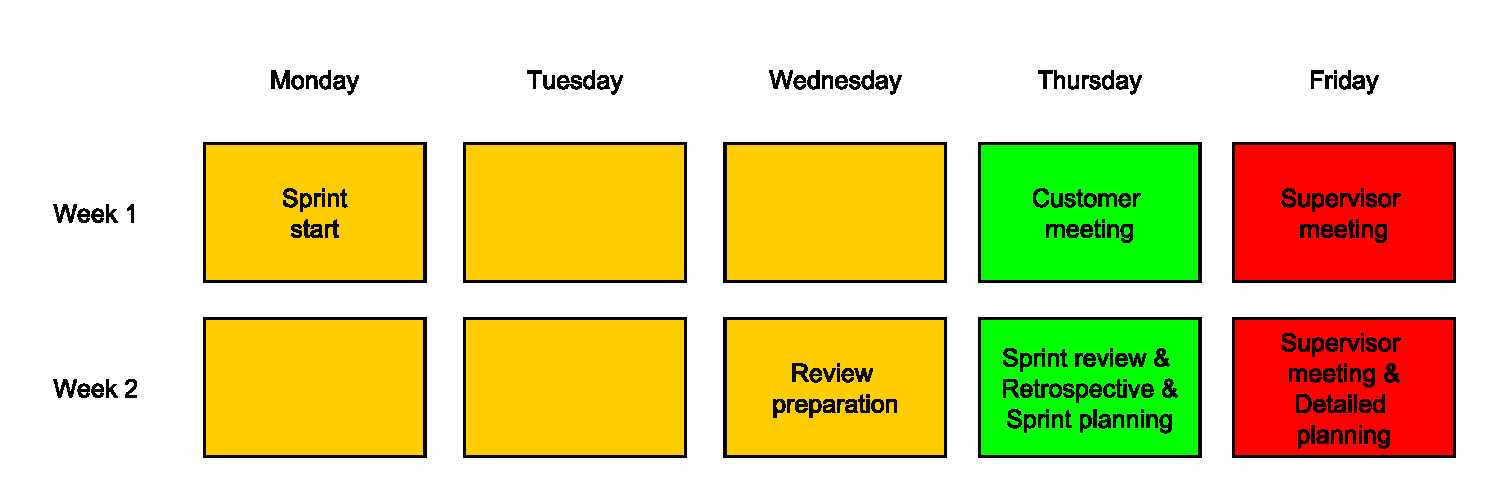
\includegraphics[scale=0.5]{images/sprint_detail.eps}
    \caption{Detailed sprint decomposition}
    \label{img:sprint_detail}
    \end{center}
\end{figure}


\paragraph{Sprint duration:}

You can see the Gantt chart depicting sprint duration and allocation into weeks in Figure \ref{fig:gantt}.
\begin{figure}[!h]
	\centering
		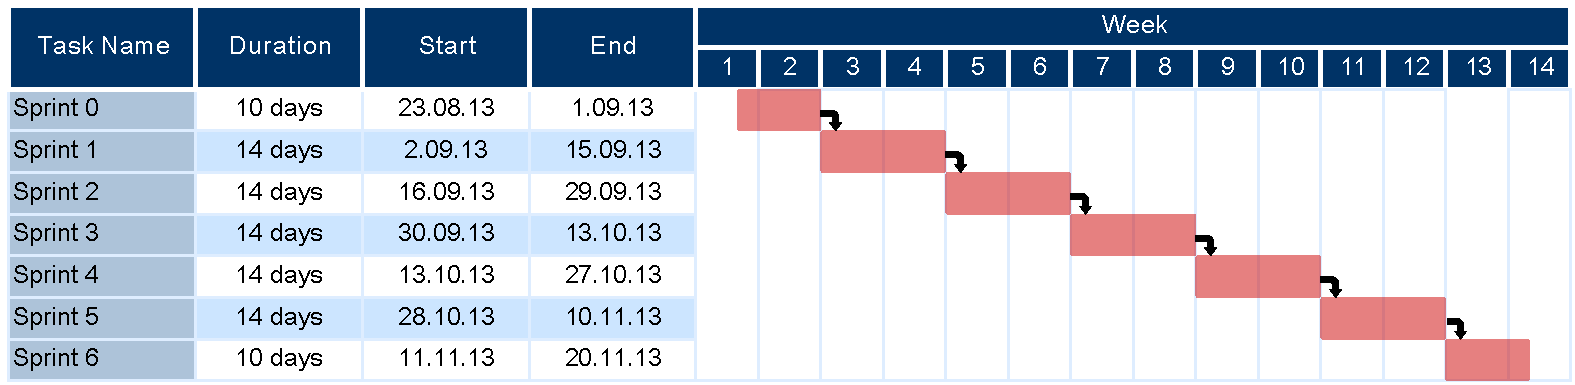
\includegraphics[width=18cm, angle=90]{planning/gantt.pdf}
	\caption{Gantt Chart}
	\label{fig:gantt}
\end{figure}

\subsection{Product Milestones}

Milestones have been set in order to more accurately determine whether or not the project is going in the right direction.
After completing some of the groups of milestones running prototypes will be delivered. 
There are 4 prototypes in total that team agreed on with the customer. 
After reaching point of 4 prototypes meeting with the customer regarding how the project is about to continue will be set. 
The last prototype implies that all milestones regarding product are reached. 
Set of milestones related to our school obligations have been set as well.

 
Overview of all milestones including 4 prototypes:

\paragraph{\"Obedient client\"  -- Prototype 1}
\begin{itemize}
	\item The server sends command to one client.
	\item The client "plays" received command (white light 10 seconds).
\end{itemize}

\paragraph{\"Obedient crowd\" -- Prototype 2}
\begin{itemize}
	\item The server sends same signal to multiple clients.
	\item The server sends multiple different commands to the clients.
	\item The client plays received commands (Red light 2 seconds, Green light 2 seconds).
\end{itemize}

\paragraph{\"I see light\" -- Prototype 3}
\begin{itemize}
	\item Server identifies one client from light.
	\item Server maps one client to grid (4 quads).
\end{itemize}

\paragraph{\"Traffic light control\" -- Prototype 4}
\begin{itemize}
	\item Server identifies multiple clients from light.
	\item Server maps all devices to the grid.
	\item Server plays traffic light simulation to the grid.
\end{itemize}

\paragraph{Course related milestones}
\begin{itemize}
	\item Finish of Project Plan document.
	\item Learn about team dynamics.
	\item Deliver Report draft.
\end{itemize}

\section{Test plan}
The purpose of this chapter is to introduce the overall plan for the testing of our product, and it describes the scope of the overall testing.
In this section there will be explained how the testing of the product was planned, who will be responsible for it, and very short mention the test criteria.
This is the strategy that will be used to verify and ensure that the product meets its requirements, and of course the quality attributes. 

\subsection{Approach}

This is a proof of concept project. The customer did not want the team to focus on the testing part on this project, but in order to deliver a valid product it will be necessary to do some testing. In order to save time and spend most of the working hours on the implementation, the black box testing will be used.  

The happy path is utilized. A happy path is a default scenario featuring no exceptional or error conditions, and comprises the sequence of activities executed if everything goes as expected. Happy path testing is a well-defined test case that uses known input, that executes without exception and that produces an expected output. This means that the team do not spend time actually writing tests, but still it must be manually tested that the product does what it is supposed to.

Verification and validation testing is also done. 
This is the process of checking that the product meets specifications, and that it fulfills its intended purpose. It may also be referred to as software quality control, and it is high-level checking. 
This will be done with test cases, or scenario testing. 
A test case is a set of conditions or variables under which a tester will determine whether an application, or one of its features, is working as it was originally established to do. 
The mechanism for determining whether a system has passed or failed such a test is known as a test oracle. 
In the case of Digital Lighter product these will be the requirements, or the use cases. Scenario testing is similar, but test cases tests single steps, and scenarios covers a number of steps. 
The scenarios should be easy to evaluate. 
The development team will not implement tests, but the tests  mus be performed manually. 
In each sprint test scenarios will be designed where the expected results with the actual result will be compared.
The integration between the deliveries in the different sprints will also have to be manually tested. 

For user testing the service TestFlight is used. TestFlight allows the customer to easily access the applications, and try out the features. The team can also get feedback from other end-users, and this way the product can be improved.  


\subsection{Responsibilities}
The whole development team is responsible for testing the product. 
Each person is responsible for testing the features they have implemented. It is important to test continuously throughout the sprints, and it will be done when the relevant functionality is implemented. The test will be performed at a time that allows the developers to fix bugs before the sprint has ended.
The person who coded specific part should not test it, rather the different person who worked on something different should perform the tests. 
This is mostly for the usability of the product. The manpower and time is limited, which means the team cannot guarantee that this is always the case.
 

\subsection{Test criteria} 

The product should function according to customer's requirements \ref{txt:requirements} and approved testing mock data.
Approval of tests and project validity will be done by customer's approval scenarios. 
Those can be images, a video, or sequence of activities that will lead to specific result. 
Test can be considered to be valid if expected result is associated with one of the mentioned approval tests.

In order to be considered successful, test execution needs to have the output as expected. 
Deviating from expected will help team in finding bugs and errors.
Confirming the expected output, since black box method is used, will be enough proof of working code.
